\begin{figure}[H]
    \centering
    \begin{subfigure}{0.47\columnwidth}
        \centering
        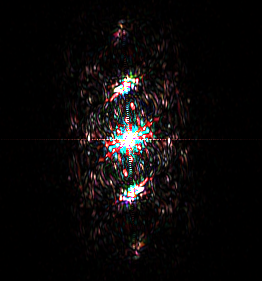
\includegraphics[width=\columnwidth]{figures/expantion fourie transform magnified.png}
        \caption{Inverse data}
        \label{fig:expansion fourie transform magnified}
    \end{subfigure}
    \centering
    \begin{subfigure}{0.49\columnwidth}
        \centering
        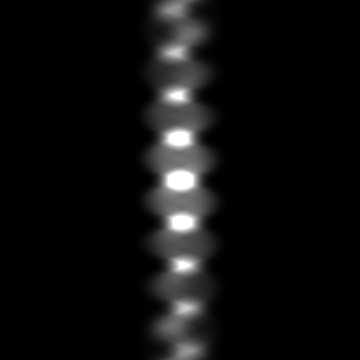
\includegraphics[width=\columnwidth]{figures/reverse fourie transform.png}
        \caption{inverse model}
        \label{fig:helix inverse fourier}
    \end{subfigure}
    \caption{Inverse discrete fourier transform calculated from the interference pattern of the helix(magnified) compared to the inverse fourier transform of the modeled helix}
    \label{fig:expansion theory measurements}
\end{figure}
